%Ich habe hie nur mal zu testzwecken einen sinnlosen Kommentar eingefuegt!
\documentclass[a4paper,10pt,notumble]{leaflet}
\usepackage[utf8]{inputenc}

\usepackage[scaled]{helvet}
\renewcommand\familydefault{\sfdefault} 
\usepackage[T1]{fontenc}
\usepackage[ngerman]{babel}
%\usepackage{setspace}
\usepackage{hyperref}
\usepackage{siunitx}
\sisetup{locale = DE}
\DeclareSIUnit[number-unit-product = { } ]
	\EUR{EUR}

\usepackage{graphicx}
\graphicspath{{gfx/}}

\newcommand{\meal}[4]{\textbf{#1}\hspace{3mm}%
\begin{minipage}[t]{5.5 cm}
\begin{flushleft}
#2\textsuperscript{#3}
\end{flushleft}
\end{minipage}%
\hfill\SI{#4}{\EUR}\newline}

% Allergen-Verzeichnis
\newcommand{\Getreideprodukte}{a}
\newcommand{\Fisch}{b}
\newcommand{\Krebstiere}{c}
\newcommand{\Schwefel}{d} 
\newcommand{\Sellerie}{e} 
\newcommand{\Laktose}{f} 
\newcommand{\Sesamsamen}{g} 
\newcommand{\Nuss}{h} 
\newcommand{\Eier}{i} 
\newcommand{\Lupinen}{j} 
\newcommand{\Senf}{k} 
\newcommand{\Soja}{l} 
\newcommand{\Weichtiere}{m} 
\newcommand{\Erdnuss}{n} 




\begin{document} 
\hypersetup{
  pdftitle={Speisekarte Yen Yen},  
  pdfsubject={Speisekarte},
  pdfauthor={Jonas Stein}
  pdfnewwindow=true
}

\begin{center}

\includegraphics[width=\textwidth]{gfx/yenyen_head}

\includegraphics[width=\textwidth]{gfx/Asia_Spezialitaeten}
\end{center}

% {\Huge Yen Yen Asia Express}\\
{\small Stand vom \today}\\[5mm]
Unser Restaurant hat an Sonn- und Feiertagen geschlossen. Reservierungen und Vorbestellungen für Selbstabholer unter
\begin{center}
{\Huge 02241 / 126 87 72}
\end{center}

\textbf{Alle Gerichte werden ohne Glutamat zubereitet.}

\section*{Erste Stärkung}
diese Gerichte sind \textbf{schnell} zubereitet und 
\textbf{auch als Vorspeise oder Hauptgericht} sehr beliebt
\begin{flushleft}
\meal{X1}{6 Mini-Frühlingsrollen, süßsauer}{\Getreideprodukte, \Soja}{2.00}
\meal{X2}{Pekingsuppe}{\Eier, \Getreideprodukte}{2.00}
\meal{X3}{Gebratener Reis mit Gemüse und Hühnerfleich}{\Soja \Eier \Getreideprodukte}{4.90}
\meal{X4}{Gebratene Nudeln mit Gemüse und Hühnerfleich}{\Soja \Eier \Getreideprodukte}{4.90}
\meal{X5}{Krabbenchips}{\Krebstiere, \Fisch, \Getreideprodukte}{1.50}
\meal{X6}{Vegetarische Krabbenchips aus Suesskartoffeln}{\Getreideprodukte}{1.90}
\meal{X7}{Gebackene Wantan, süßsauer}{\Eier, \Soja,\Getreideprodukte,\Sellerie}{2.90}
\meal{X8}{Gebackener Brokkoli}{\Soja,\Getreideprodukte,\Sellerie,\Eier}{2.90}
\end{flushleft}

\section*{Vorspeisen}
\meal{U1}{Zwei vietnamesische Frühlingsrollen, hausgemacht, süßsauer}{\Getreideprodukte, \Soja, \Eier, \Sellerie}{3.50}
\meal{U2}{Zwei vietnamesische Frühlingsrollen, hausgemacht, pikant}{\Getreideprodukte, \Soja, \Eier, \Sellerie}{3.50}
\meal{U3}{Eine chinesische Frühlingsrolle, hausgemacht, süßsauer}{\Getreideprodukte, \Soja, \Eier, \Sellerie}{3.20}
\meal{U4}{Eine chinesische Frühlingsrolle, hausgemacht, pikant}{\Getreideprodukte, \Soja, \Eier, \Sellerie}{3.20}

\section*{Suppen}
\meal{Z1}{Pekingsuppe mit Hühnerfleich}{\Soja,\Getreideprodukte,\Sellerie,\Eier}{2.00}
\meal{Z2}{Wantansuppe}{\Soja,\Getreideprodukte,\Eier}{2.90}
\meal{Z3}{Gemüsesuppe mit Hühnerfleich}{\Soja}{3.50}
\meal{Z4}{Gemüsesuppe mit Glasnudeln}{\Soja\Getreideprodukte}{3.50}
\meal{Z5}{Vegetarische Gemüsesuppe mit Tofu}{\Soja\Getreideprodukte\Lupinen}{3.90}


\section*{Hühnerfleisch}
\meal{H1}{gebraten mit gebratenem Reis}{\Getreideprodukte,\Eier,\Soja}{4.90}
\meal{H2}{gebraten mit gebratenen Nudeln}{\Getreideprodukte,\Eier,\Soja}{4.90}

\meal{H3}{gebraten in Currysoße mit Kokosmilch}{\Laktose, \Getreideprodukte}{6.90}
\meal{H4}{auf Thai Art, scharf mit Kokosmilch}{\Getreideprodukte, \Soja}{6.90}
\meal{H5}{gebraten mit Bambus und Morcheln}{\Getreideprodukte, \Soja}{6.90}
\meal{H6}{gebraten mit Gemüse der Saison}{\Getreideprodukte, \Soja}{6.90}
\meal{H7}{im Teigmantel gebacken mit Gemüse und Reis, süßsauer}{\Eier \Getreideprodukte, \Soja, \Sellerie}{6.90}
\meal{H8}{im Teigmantel gebacken mit Gemüse und Reis, pikant}{\Eier \Getreideprodukte, \Soja}{6.90}

\meal{H9}{gebraten mit Gemüse in süßsaurer Soße}{\Getreideprodukte, \Sellerie}{6.90}

\meal{H10}{gebraten mit Gemüse und Reis, pikant}{\Getreideprodukte, \Soja}{6.90}

\meal{H11}{Kung Bao art, pikant}{\Getreideprodukte, \Nuss, \Soja}{6.90}

\meal{H12}{mit Brokkoli und Knoblauch}{\Getreideprodukte, \Nuss, \Soja}{6.90}

\meal{H13}{mit Ingwer und Zitronengras}{\Getreideprodukte, \Soja}{6.90}
%Thịt nướng xâu
\meal{H14}{als Saté Spieße süßsauer}{\Getreideprodukte, \Sellerie}{7.90}
\meal{H15}{als Saté Spieße mit Erdnußsoße}{\Getreideprodukte, \Soja, \Erdnuss, \Laktose}{8.90}
\meal{H16}{als Saté Spieße mit spezial Hoisin-Sauce}{\Getreideprodukte, \Soja, \Sesamsamen, \Laktose}{8.90}


\section*{Spezialitäten vom Rind}
zartes Rinderfilet in Streifen geschnitten und kurz angebraten
\begin{flushleft}
\meal{R1}{pikant mit Reis}{\Getreideprodukte, \Soja}{7.90}
\meal{R2}{mit Zwiebeln und Sellerie und Reis}{\Getreideprodukte, \Soja, \Sellerie}{7.90}
\meal{R3}{mit chinesischen schwarzen Bohnen und Reis}{\Getreideprodukte, \Soja, \Laktose}{7.90}
\meal{R4}{mit Zitronengras und Reis}{\Getreideprodukte, \Soja}{7.90}
\meal{R5}{mit Gemüse und Reis}{\Getreideprodukte, \Soja}{7.90}
\meal{R6}{mit Champignons, Zwiebeln und Reis}{\Getreideprodukte, \Soja}{7.90}
\meal{R7}{Thai Art mit Kokosmilch, scharf}{\Laktose}{8.90}
\end{flushleft}

\section*{Kross gebratenes Entenbrustfilet}
in einer knusprigen Hülle frisch gebraten serviert
\begin{flushleft}
\meal{E1}{mit Gemüse und süßsaurer Soße}{\Senf,\Erdnuss}{8.90}
\meal{E2}{mit Gemüse und pikanter Soße}{\Senf,\Erdnuss}{8.90}
\meal{E3}{mit Gemüse und Erdnuss Soße}{\Senf,\Erdnuss}{9.90}
\meal{E4}{mit Gemüse und Thaisoße}{\Senf,\Erdnuss}{9.90}
\end{flushleft}

\section*{Spezialitäten aus dem Wasser}
\begin{flushleft}
\meal{W1}{Norwegischer Premium Lachs mit Gemüse der Saison}{\Fisch, \Getreideprodukte, \Soja, \Krebstiere}{9.90}
\meal{W2}{Norwegischer Premium Lachs mit Gemüse der Saison in Curry-Soße}{\Fisch, \Getreideprodukte, \Laktose, \Krebstiere}{11.90}
\meal{W3}{Norwegischer Premium Lachs mit Kung Bao-Soße}{\Fisch, \Getreideprodukte, \Laktose, \Nuss, \Soja}{11.90}
\meal{W4}{Garnelen Kung Bao Art, scharf}{\Fisch, \Getreideprodukte, \Soja, \Nuss, \Krebstiere}{8.90}
\meal{W5}{Garnelen im Teigmantel}{\Eier \Fisch, \Getreideprodukte, \Soja, \Laktose, \Krebstiere}{8.90}
\meal{W6}{Garnelen mit Ingwer und Zitronengras}{\Fisch, \Getreideprodukte, \Soja, \Krebstiere}{8.90}
\meal{W7}{Garnelen mit gebratenen Nudeln}{\Fisch, \Getreideprodukte, \Soja, \Krebstiere}{8.90}
\meal{W8}{Garnelen mit mit Gemüse der Saison und Reis}{\Fisch, \Getreideprodukte, \Soja, \Krebstiere}{8.90}
\end{flushleft}

\section*{Yen-Yen Menue}
\meal{Y1}{Ueberaschungsgericht}{\Laktose, \Getreideprodukte, \Soja, \Nuss, \Sesamsamen, \Sellerie}{8.90}
\meal{Y2}{Ueberaschungsgericht mit Ente}{\Laktose, \Getreideprodukte, \Soja, \Nuss, \Sesamsamen, \Sellerie}{9.90}


\section*{Extras} 
\meal{+R}{gebratenen Reis als Beilage extra}{~}{1.80}
\meal{+N}{gebratene Nudeln als Beilage extra}{~}{1.80}
\meal{+S}{auf Wunsch bereiten wir Ihr Gericht scharf zu}{\Fisch}{0.00}

\section*{Für kreative}
Stellen Sie sich Ihr Lieblingsgericht aus folgenden Zutaten selbst zusammen:
Reis, gebratene Nudeln, Bambus, Brokkoli, Cashewkerne, Ingwer, Zwiebeln, Knoblauch,
Rindfleisch, gebratene Ente, Hühnerfleisch

\section*{Nachspeisen} 
\meal{N1}{frisch gebackene Banane mit Honig}{\Getreideprodukte, \Eier}{2.50}
\meal{N2}{Vanilleeis mit Früchten garniert}{\Laktose}{2.90}

%\vspace{0.5cm}
%\newpage
\section*{Kalte Getränke}
\meal{G1}{Cola (0,2 L)}{~}{1.60}
\meal{G2}{Cola (0,3 L)}{~}{1.90}
\meal{G3}{Fanta (0,2 L)}{~}{1.60}
\meal{G4}{Fanta (0,3 L)}{~}{1.90}
\meal{G5}{Wasser (0,2 L)}{~}{1.60}
\meal{G6}{Wasser (0,3 L)}{~}{1.90}
\meal{G7}{Bitburger alkoholfrei}{~}{1.90}
\meal{G8}{Malzbier (0,2 L)}{~}{1.90}
\meal{G9}{Bitter Lemon (0,2 L)}{~}{1.90}
\meal{G10}{Ginger Ale (0,2 L)}{~}{1.90}
\meal{G11}{Lychee Nektar (0,2 L)}{~}{1.90}
\meal{G12}{Mangosaft (0,2 L)}{~}{1.90}
\meal{G13}{Orangensaft (0,2 L)}{~}{1.90}
\meal{G14}{Capri Sonne Trinkpackung}{~}{0.80}

\section*{Tee und Kaffee}
\meal{J1}{Kamillentee}{~}{1.90}
\meal{J2}{Jasmintee}{~}{1.90}
\meal{J3}{Drachenperlen (Jasmin Tee)}{~}{2.50}
\meal{J4}{Schwarzer Tee}{~}{1.90}
\meal{J5}{Blumentee (Kännchen)}{~}{1.90}
\meal{J6}{Kaffee}{~}{1.90}
\meal{J7}{Cappuchino}{~}{1.90}

\section*{Alkoholische Getränke}
\meal{V1}{Gaffel Kölsch (0,2 L)}{~}{1.90}
\meal{V2}{Bitburger Pils}{~}{1.90}
\meal{V3}{Paulaner Weizen (0,5 L)}{~}{2.90}
\meal{V4}{Pflaumenwein (0,04 L)}{~}{2.50}
\meal{V5}{Rotwein}{~}{4.90}
\meal{V6}{Weißwein}{~}{4.90}

\section*{Partyservice}
Sie möchten Ihre Gäste in Ihrer Location mit gesunden, asiatischen Speisen verwöhnen?\\ 
Sprechen Sie uns an, wir beraten Sie gern.


%\newpage
\section*{Allergenkennzeichnung}
\begin{verbatim}
nach EU-Lebensmittelinformationsverordnung
a Getreideprodukte (Glutenhaltig) 
b Fisch
c Krebstiere
d Schwefeldioxide und Sulfite 
e Sellerie
f Milch und Laktose
g Sesamsamen
h Nüsse
i Eier
j Lupinen
k Senf
l Soja
m Weichtiere
n Erdnüsse
\end{verbatim}
Informationen über Zutaten in unseren Speisen, die Allergien
oder Unverträglichkeiten auslösen können, erhalten Sie auf Nachfrage
auch bei unseren Mitarbeitern.\\ 
\textbf{Gerne passt unser Koch das Rezept auf Ihre Bedürfnisse an.} %
%\newpage
%\section*{Lage in der Troisdorfer Innenstadt}
\begin{center}
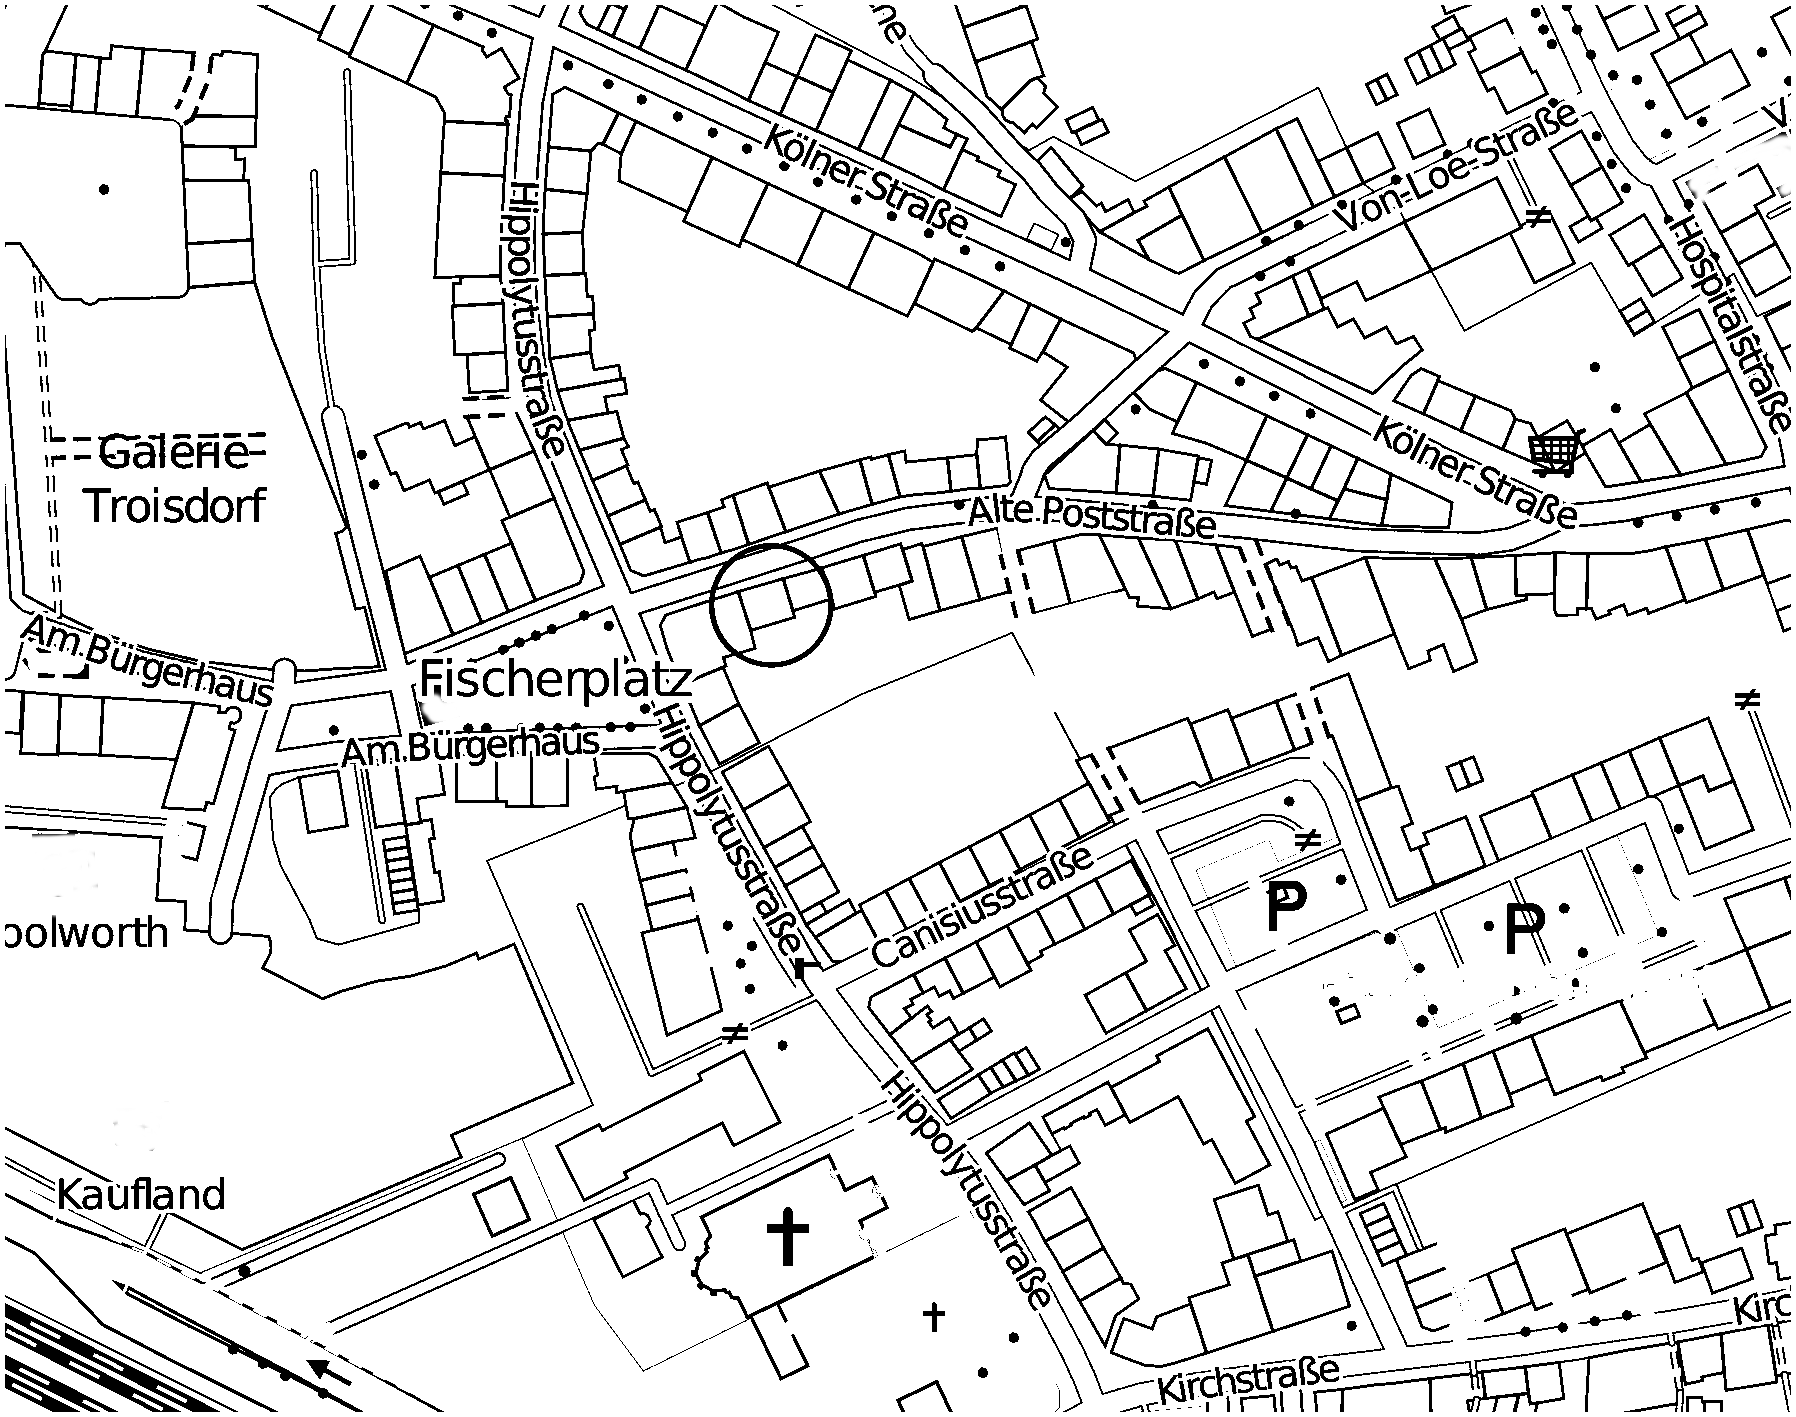
\includegraphics[width=0.7\textwidth]{gfx/map/rect28239c}\\
Alte Poststraße 34, 53840 Troisdorf

Inhaber Tien Long Nguyen\hfill http://www.yen-yen.de/
\end{center}

\end{document}